% !TeX root = ../document_maitre.tex

Les deux axes d'améliorations que nous venons de distinguer sont pensés en deux outils distincts. La \guillemet{recherche augmentée} : une recherche assistée par \gls{IA} pour interroger le \gls{SRI} en langage naturel. Et un \guillemet{\gls{chatbot}} pour disposer d'un guide et d'un appui au contrôle des données. Ces outils puisent dans la même source technologique mais sont des processus divergents à portées différentes. Ainsi, ils font l'objet d'interfaces différenciées.

Il existe aujourd'hui quelques projets et travaux académiques sur ces deux sujets. Ils ne sont pas nombreux et recouvrent des réalités techniques et professionnelles différentes aux nôtres. Il convient donc de présenter des états de l'art de chaque outil, à l'aide de ses connaissances, afin d'analyser les réalités techniques se cachant derrière ces fonctionnalités. Cela amène à des discussions sémantiques afin de lever des confusions terminologiques et techniques importantes, notamment autour du \gls{chatbot}. Nous en profiterons pour discerner les apports, limites et enjeux des technologies et processus cités.

\subsection{La \guillemet{recherche augmentée} : }

\subsubsection{La recherche intelligente}


L'origine de ce processus est la recherche intelligente, mis en place par les grands moteurs de recherche afin d'offrir des résultats pertinents sous forme de résumé.\footcite{flamentGoogleSGEAI2025}. Il vise à augmenter l'accessibilité utilisateur grâce au langage naturel et à offrir des résultats plus pertinents par l'interprétation de la phrase.\footcite{flamentGoogleSGEAI2025}. Fondement du reste de notre travail, il convient de l'explorer. Trois outils d'\gls{IA} le compose : le \gls{LLM}, le \gls{RAG} et les modèles de \gls{NLP}.\newline

Le \gls{LLM} constitue l'intermédiaire entre les données et l'utilisateur. Basé sur du \gls{DPL}, il mobilise les technologies du \gls{NLP} et les combine a une faculté de raisonnement. De cette manière, il est capable d'analyser et d'extraire la sémantique d'une phrase mais aussi de formuler ses propres phrases. Dans ce processus, il intervient au moment de la réponse afin de converser avec l'utilisateur. 
Pour cela il extrait des \glspl{tk}, c'est à dire des mots, de nos phrases qui sont analyser par différents processus de \gls{NLP}. Ils sont ensuite transformés en \gls{vcs}, une suite de chiffre unique, qui lui permettent de faire des liens sémantique et de \guillemet{comprendre}.

Le \gls{RAG} est le procédé au \coeur du processus car il permet de fiabiliser et contextualiser les résultats, réduisant les hallucinations des \glspl{LLM}. En effet, ce dernier peut parfois répondre à l'aide de ses propres \guillemet{connaissances} ce qui créer des éléments de réponses faussés. En connectant un \gls{LLM} à une ou plusieurs bases de données, on créer une source de connaissances vérifiée et validée par un opérateur humain sur laquelle il est contraint de s'appuyer. Pour répondre, le \gls{LLM} doit les analyser et les reformuler.\footnote{Pour plus d'informations sur le \gls{RAG} voir \pageref{rag}}

Les modèles de \gls{NLP} sont spécialisés sur des tâches précises telles que le \gls{POS} et le \gls{NER}. Ils sont appliqués successivement afin de mieux saisir le besoin profond exprimé dans une requête. Mais aussi de mieux comprendre les données stockées. Cela augmente la qualité de la \gls{Vecsion} et donc la pertinence des réponses. 

La combinaison de ces trois éléments permet de créer la recherche intelligente. On peut distinguer deux temps dans son fonctionnement. Le premier temps est une phase d'analyse, invisible par l'utilisateur. En voici un schéma :

\begin{figure}[H] \label{procrag}
\centering
\begin{tikzpicture}[
node distance=1.2cm,
% Définition directe des styles à l'intérieur de l'environnement tikzpicture
stepbox/.style={
rectangle,
draw=blue!80!black,
fill=blue!5,
thick,
rounded corners=4pt,
minimum width=9.5cm,
minimum height=1.2cm,
align=center,
font=\sffamily
},
arrow/.style={
->,
>=Stealth,
very thick,
draw=blue!80!black
}
]

% --- 1. LES SOURCES ---
\node (sources) [font=\sffamily\small, align=center, text=gray!80!black] 
{Sources de données : \textit{(PDF, Base de données, ...)}};

% --- 2. LES 4 ÉTAPES CLÉS ---
\node (e1) [stepbox, below=0.8cm of sources] {
\textbf{1. Connexion à la source de données}\\
\small Connecte l'outil aux données stockées.
};

\node (e2) [stepbox, below=of e1] {
\textbf{2. Analyse sémantique par modèle de \gls{NLP}}\\
\small \gls{POS}, \gls{NER}, \dots
};

\node (e3) [stepbox, below=of e2] {
\textbf{3. Indexation unifiée des données}\\
\small Réunis les données en un index permettant de classer les données.
};

\node (e4) [stepbox, fill=green!15, draw=green!60!black, below=of e3] {
\textbf{4. \Gls{Vecsion} des données indexées}\\
\gls{vcs} calculés à partir des données indexées.
};

% --- 3. FLÈCHES DE LIAISON ---
\draw [arrow] (sources) -- (e1);
\draw [arrow] (e1) -- (e2);
\draw [arrow] (e2) -- (e3);
\draw [arrow] (e3) -- (e4);

\end{tikzpicture}
\caption{Phase d'analyse de la recherche intelligente.}
\end{figure}

\newpage

Ce que l'on voit ici est principalement le mécanisme du \gls{RAG}. Une fois connectés à une source de données, il l'analyse grâce aux modèles de \gls{NLP}. Ainsi, on donne du sens sémantique à ces données dès lors considérées comme \guillemet{enrichies}. Elles sont ensuite réunies dans un index : comme un \gls{SRI}\footnote{Voir \fullref{Keyword}} le \gls{RAG} dispose de sa propre architecture de données. C'est sur cet index que la \gls{Vecsion} s'applique, créant des \gls{vcs} qui sont légers, plus faciles à interroger et plus fiables que l'index des données. Cela crée un double avantage par rapport à une recherche par mots-clés traditionnels. D'abord, une compréhension sémantique des données et ensuite une rapidité dans leur interrogation. En théorie, nos résultats gagnent en précision et rapidité.\newline

L'envoi d'une requête utilisateur formulée en langage naturel déclenche une nouvelle phase de traitement qui suit les étapes suivantes : 


\begin{figure}[H]
\centering
\begin{tikzpicture}[
node distance=1cm,
% Style des blocs standards
box/.style={
rectangle,
draw=blue!80!black,
fill=blue!5,
thick,
rounded corners=3pt,
minimum width=8.5cm,
minimum height=1.1cm,
align=center,
font=\sffamily\small
},
% Style des flèches
arrow/.style={
->,
>=Stealth,
very thick,
draw=blue!80!black
}
]

% --- LES ÉTAPES DU FLUX ACTIF ---

\node (e1) [box] {
\textbf{1. Réception de la requête}\\
\small Saisie de la requête en langage naturel
};

\node (e2) [box, below=of e1] {
\textbf{2. Analyse par NLP}\\
\small \gls{POS}, \gls{NER}, \dots
};

\node (e3) [box, below=of e2] {
\textbf{3. Vectorisation en direct}\\
\small Transformation de la demande en \gls{vcs}
};

\node (e4) [box, fill=purple!10, draw=purple!80!black, below=of e3] {
\textbf{4. Comparaison sémantique}\\
\small Mise en correspondance du \gls{vcs} de la requête aux \glspl{vcs} des données stockées.
};

\node (e5) [box, fill=green!15, draw=green!60!black, below=of e4] {
\textbf{5. Restitution des résultats}\\
\small Tri et affichage des réponses les plus pertinentes
};

% --- FLÈCHES DE LIAISON ---
\draw [arrow] (e1) -- (e2);
\draw [arrow] (e2) -- (e3);
\draw [arrow] (e3) -- (e4);
\draw [arrow] (e4) -- (e5);

\end{tikzpicture}
\caption{Phase dite \guillemet{active} de la recherche intelligente.}
\end{figure}

\vspace{0.1cm}

La phase \guillemet{active} de ce processus débute à l'envoi par l'utilisateur d'une requête en langage naturel. Ensuite on applique le même principe que précédemment : on comprend d'abord sémantiquement la requête à l'aide de modèles de \gls{NLP} avant d'opérer une \gls{Vecsion} des données composant la requête.

Ce sont les \glspl{vcs} qui sont ensuite comparés : des vecteurs proches signifient des correspondances sémantiques. Alors on vient chercher le sens profond de la donnée : l'idée qu'elle exprime. De cette manière on crée la capacité à saisir les idées représentées par les mots à une volonté. On ne s'arrête plus à la simple correspondance typographique.

Voici un schéma représentant le fonctionnement final d'un processus de recherche intelligente : 

\begin{figure}[H]
\centering
\begin{tikzpicture}[
node distance=0.9cm and 1.2cm,
% Définition des blocs et des flèches utilisées dans le schéma
box/.style={
rectangle,
draw=blue!80!black,
fill=blue!5,
thick,
rounded corners=3pt,
minimum width=6.5cm,
minimum height=1cm,
align=center,
font=\sffamily\small
},
passivebox/.style={
rectangle,
draw=orange!80!black,
fill=orange!5,
thick,
rounded corners=3pt,
minimum width=4.5cm,
minimum height=1cm,
align=center,
font=\sffamily\small
},
database/.style={
cylinder,
cylinder uses custom fill,
cylinder end fill=blue!20,
cylinder body fill=blue!10,
draw=blue!80!black,
thick,
aspect=0.25,
minimum width=3cm,
minimum height=1.2cm,
align=center,
font=\sffamily\small\bfseries
},
arrow/.style={
->,
>=Stealth,
very thick,
draw=blue!80!black
},
passivearrow/.style={
->,
>=Stealth,
very thick,
draw=orange!80!black,
dashed
}
]


% Phase d'analyse, située sur la gauche

\node (docs) [passivebox] {Données stockées\\(PDF, Bases de données, \dots)};
\node (doc_vec) [passivebox, below=of docs] {Extraction du sens par \gls{NLP} \\ et Vectorisation des données};
\node (index) [database, below=1.2cm of doc_vec] {Index de \glspl{vcs}\\des données stockées};

% Phase de requêtage, située sur la droite

\node (req) [box, right=2.5cm of docs] {1. Réception de la requête\\en langage naturel};
\node (nlp) [box, below=of req] {2. Analyse \gls{NLP} pour extraction du sens};
\node (vec) [box, below=of nlp] {3. \Gls{Vecsion} de la requête};
\node (comp) [box, fill=purple!10, draw=purple!80!black, below=of vec] {4. Comparaison des \glspl{vcs}\\ de la requête et de l'index};
\node (res) [box, fill=green!15, draw=green!60!black, below=of comp] {5. Retour des résultats pertinents \\ sur proximité des \glspl{vcs}};

% Création des flèches entre les blocs et phases

\draw [passivearrow] (docs) -- (doc_vec);
\draw [passivearrow] (doc_vec) -- (index);

\draw [arrow] (req) -- (nlp);
\draw [arrow] (nlp) -- (vec);
\draw [arrow] (vec) -- (comp);
\draw [arrow] (comp) -- (res);

\draw [arrow, draw=purple!80!black] (index) -- (comp) 
node[midway, above, font=\sffamily\tiny, text=purple!80!black] {Mise en correspondance};

% Définitions des cadres de regroupement
\node[draw=orange!80!black, dashed, thick, rounded corners, fit=(docs) (doc_vec) (index), 
inner sep=8pt, label=above:{\sffamily\bfseries\color{orange!80!black}I. Phase d'analyse}] {};

\node[draw=blue!80!black, thick, rounded corners, fit=(req) (nlp) (vec) (comp) (res), 
inner sep=8pt, label=above:{\sffamily\bfseries\color{blue!80!black}II. Phase de requêtage}] {};

\end{tikzpicture}
\caption{Fonctionnement global de la recherche intelligente.}
\end{figure}

Ce que nous avons décrit ici est un processus générique généralement modifié. Le \gls{chck} par exemple, permettant de fractionner des documents en plusieurs morceaux. Cela permet d'accélérer le traitement par la parallélisation de tâches\footnote{Désigne en informatique la capacité à traiter simultanément plusieurs tâches et données parfois dans des processus différents.} et de limiter la perte de précision par des analyses restreintes. Ce n'est qu'après qu'on peut extraire des \gls{tk}.\footcite{QuestceQueChunking} 

Ou encore le \gls{RR}. À l'issue du processus générique, les résultats les plus pertinents sont sélectionnés et classés selon un ordre d'importance. Le \gls{LLM} l'utilise afin d'organiser sa réponse. Cet outil consiste à évaluer la pertinence des résultats et les reclasser. Il effectue sa propre recherche dans les données stockées et les compare à la requête utilisateur, en fonction des divergences il refait un classement si besoin.\footcite{ultralyticsQuestCeQuun2026}\newline

Les limites restent importantes et mettent en doute la qualité scientifique des résultats. L'utilisation d'\gls{IAG} entraîne le risque d'hallucination et le \gls{RAG} limite mais n'annule pas ce risque. Notamment sur des requêtes basées sur des expressions imagées ou des termes spécifiques à des \guillemet{jargons} professionnels. Si le sens n'est pas saisi, il sera halluciné afin de créer une réponse tout de même.\footcite{cazzaroQueryingLLMsIf} 

De plus, ce processus ne peux procéder à des calculs d'agrégation de données. Ainsi, on en peut avoir recours à des calculs comme des moyennes, ce qui est essentiel dans certains domaines de recherches. \footcite{cazzaroQueryingLLMsIf} 

Ajoutons que la segmentation des documents par \gls{chck}, souvent utilisé, apporte des limites aux recherches complexes. Morceler les documents revient à multiplier les points d'informations et donc les calculs. Lorsqu'une requête amène à analyser un grand nombre de segments, le \gls{RAG} peut entrer dans un état de confusion et générer du bruit.\footcite{cazzaroQueryingLLMsIf} 

De plus, la recherche intelligente n'est pas transparente quant aux modalités de recherche. Le \gls{RAG} et le \gls{LLM} ne sont pas transparents dans leurs opérations et processus de réflexion. Ainsi, des doutes peuvent exister : a-t-il confondu des termes ? A-t-il halluciné ? A-t-il mal compris ? Toutes ces questions restent sans réponse et créent le même problème rencontré avec les \gls{SRI}\footnote{Voir page \pageref{opaque}}. 

Il y a aussi un enjeu de sécurité et de confidentialité des données. Il peut arriver que l'on souhaite ne distribuer que certaines informations à certaines personnes, ce qui est faisable grâce aux droits d'accès. Ces derniers sont difficiles à gérer sur des \gls{vcs}. Des systèmes le permettent, mais ils connaissent encore un certains nombre de faille trop importante posant le problème de la sécurité de l'information et de sa confidentialité. Deux principes clés dans nos institutions patrimoniales.

\subsubsection{Les processus \gls{2SQL} et \gls{2NSQL}}

L'objectif global est d'adapter le processus précédent aux technologies SQL et \gls{NSQL} dans des processus hybrides appelés :\gls{2SQL} ou \gls{2NSQL}. Ils présentent certains avantages :

Il n'y a pas d'hallucination : si la requête n'est pas comprise il n'y a simplement pas de réponse. Ils permettent des calculs mathématiques sur des données stockées en tant que chiffres. Et les requêtes complexes, multipliant les sources, ne sont pas sujettes à confusion grâce aux jointures pour le SQL et aux \gls{pipagreg} pour le \gls{NSQL}. Les requêtes sont compréhensibles par l'humain et re-jouable ce qui apporte une transparence au processus. Et pour finir, ils intègrent nativement des outils de contrôle des droits d'accès assurant la confidentialité des données. Le \gls{NLP} devient un outil de traduction vers le SQL ou \gls{NSQL} évitant la \gls{Vecsion} et l'interprétation de l'\gls{IA}. 

Cependant, il y a un manque considérable d'informations sur les projets menés à ce sujet dans notre domaine hors mis quelques approches spécifiques.\footnote{Nous ne développons pas ces approches plus poussées, mais les mentionnons par souci d'exhaustivité. Pour plus d'informations sur ces approches divergentes, consulter \cites{sergeevTalkingDataDesigning}{cazzaroQueryingLLMsIf}} Ainsi, nous allons expliquer de manière générale comment fonctionne un \textit{pipeline} \gls{2SQL} et \gls{2NSQL}. Commençons par mettre en exergue les trois difficultés majeures de cette adaptation : \newline 

D'abord, la compréhension des schémas SQL et du contexte métier. Les bases SQL ont une structure rigide créées sur les besoins de descriptions des institutions. Ces structures embarque des biais de recherches et d'exploitation définis selon une stratégie institutionnelle et les \guillemet{besoins métiers}\footnote{On parle de \guillemet{besoin métier} pour exprimer les besoins inhérent à un domaine professionnel et propre à ce domaine. Il correspond souvent à la réalité des pratiques employées par les professionnels.}. On attend de l'\gls{IA} qu'elle puisse comprendre un univers métier et institutionnel. On déplace ainsi le curseur de la compréhension des données stockées à celle de l'univers professionnel.\footcite{CommentObtenirCode}

Ensuite, la compréhension du besoin utilisateur. Si la recherche intelligente permet de rectifier les processus de réflexions de l'\gls{IA}, le \gls{2SQL} est moins souple sur le sujet. Pour changer cette réflexion cela demande de connaître la structuration de la base de données afin de guider le \gls{mod}. Cette compétence technique est cependant rare dans les institutions conservatrices ce qui amène le besoin de limiter les incompréhensions des requêtes et les interactions entre l'utilisateur et la base SQL.\footcite{CommentObtenirCode}

Enfin, la notion de \guillemet{[..] dialecte SQL [...]}\footcite{CommentObtenirCode}. Tout les systèmes de gestion des bases de données n'emploient pas exactement le même langage, et les \glspl{LLM} ont souvent du mal à s'adapter aux différences. Sur certains systèmes, la génération de requêtes complexes s'en trouve complexifiée et réactive le risque d'hallucination.\footcite{CommentObtenirCode}

Deux approches permettent de combler cet écart : les \textit{frameworks} spécialisés comme VANNA AI et les \gls{AGSQL} comme LangChain\footcite{TexttoSQLInterrogerVos2026}. La première approche consiste à créer un processus de \gls{RAG} avec le schéma SQL, des exemples de requêtes et de la documentation professionnelle. Ainsi, n'importe quel \gls{LLM} peut comprendre son environnement. Il atteint vite ses limites car chaque changement d'architecture de la base amène un changement de documentation et donc de résultats. La seconde approche est basée sur des \gls{LLM} spécialisé dans la compréhension et la génération de requête SQL y compris sur des bases complexes. Cet est outil est plus complexe à mettre en place et à maintenir. Qu'il soit basé sur un \gls{AGSQL} ou un \textit{framework}, un processus \gls{2SQL} ressemble à ceci :

\begin{figure}[H]
\centering
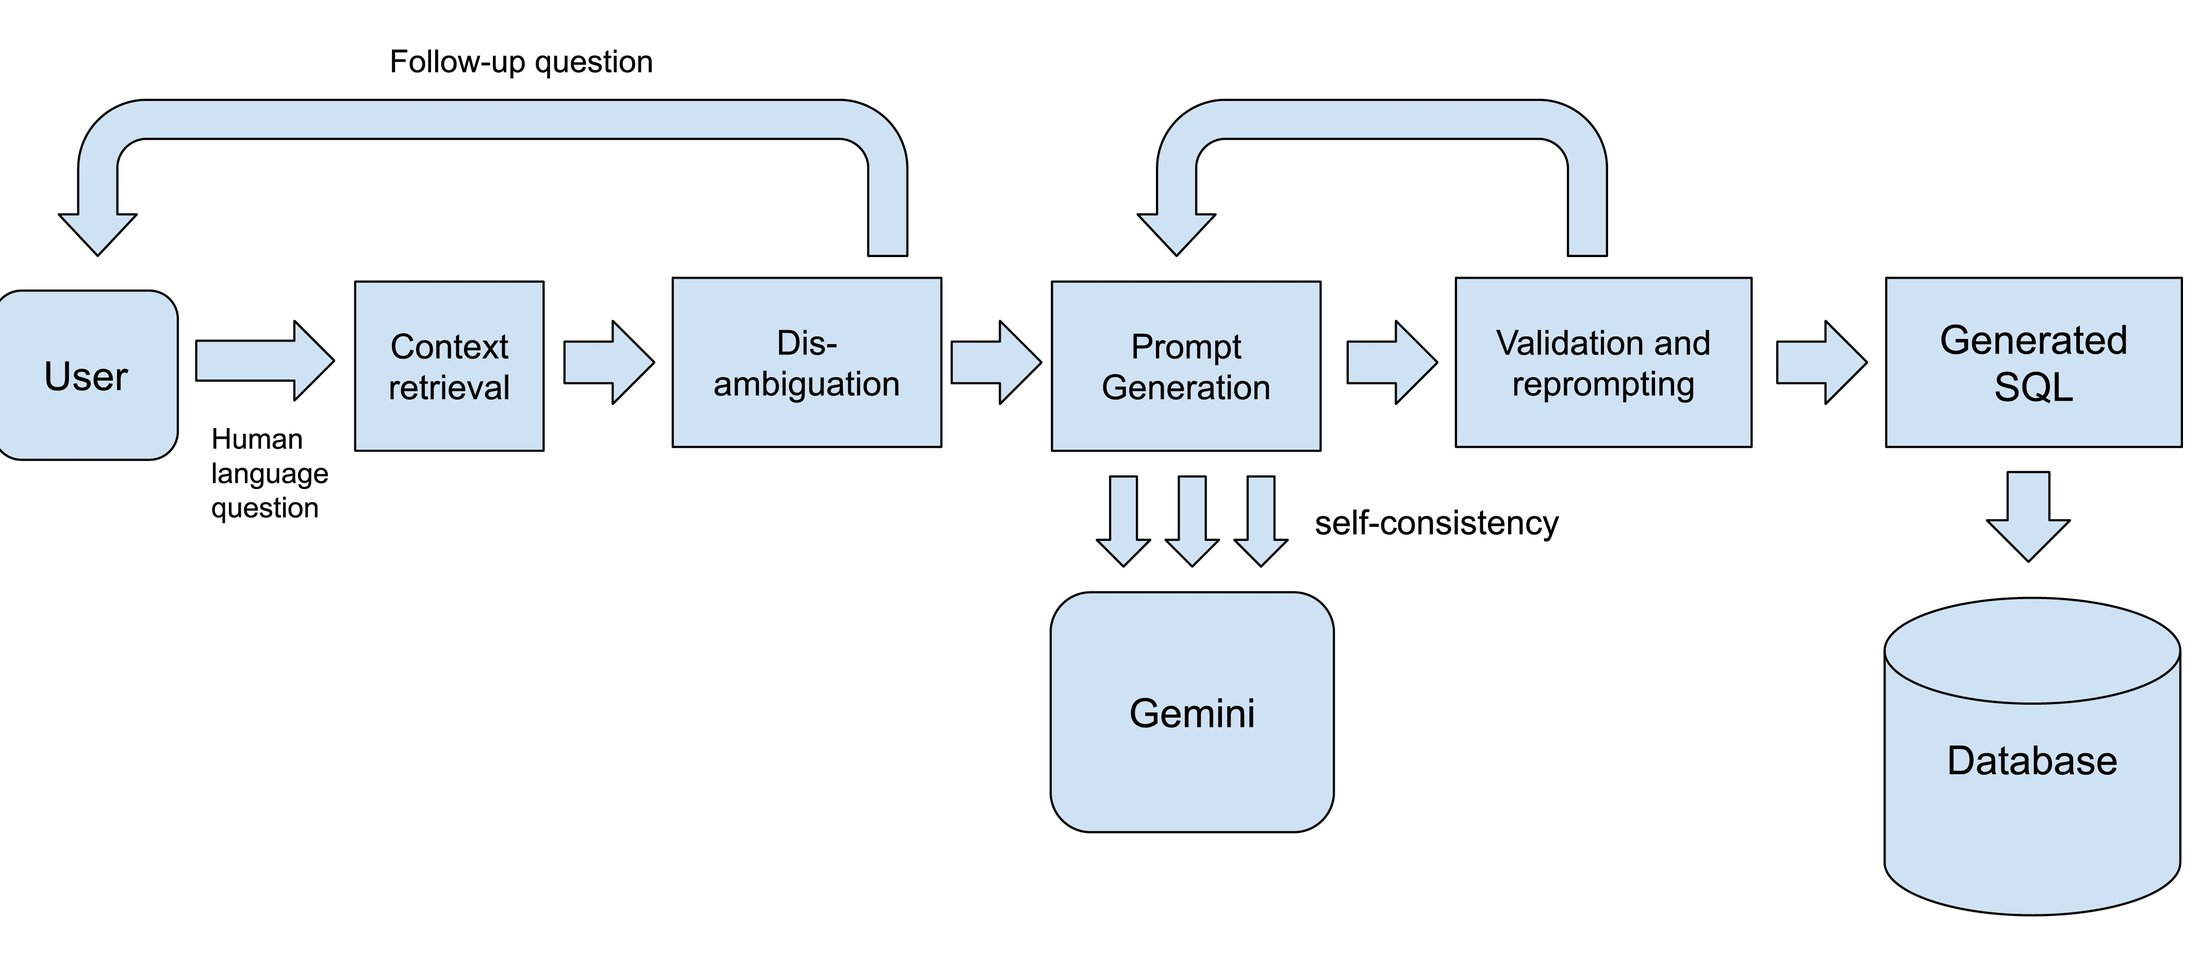
\includegraphics[width=0.8\textwidth]{./Schema/Text-to-SQL.png}
\caption{Schéma d'un pipeline \gls{2SQL}. Source : \cite{CommentObtenirCode}}
\label{fig:text-to-sql-schema}
\end{figure}

Nous en distinguons deux temps : le premier est consacré à la compréhension des besoins utilisateurs exprimés dans la requête initiale. Pour cela, on accorde la capacité au \gls{LLM} de relancer l'utilisateur à l'aide de question afin de clarifier le besoin. Il est essentiel pour cela que l'outil comprenne l’environnement métier dans lequel il s'inscrit. 

Le second temps est consacré à la génération de la requête SQL grâce au \gls{LLM}. D'abord il reformule la requête afin de la rendre plus compréhensible, augmentant la précision de la requête SQL générée. Cela donne naissance à un nouveau prompt généré par \gls{LLM} dans le seul but de générer du SQL. Ce prompt entre dans une boucle de traitement : il est examiné, puis soit refusé et reformulé soit validé ce qui entraîne la génération d'une requête SQL et son envoi à un \guillemet{parseur SQL}, un logiciel de vérification syntaxique des requêtes SQL. Cette requête est ensuite directement adressée à la base SQL en question. Dans le cas où l'institution possède plusieurs bases de données, le \gls{2SQL} peut s'y adapter. Soit par l'intégration d'un moteur de recherche fédéré, déclinant la requête selon l'architecture propre à chaque base, soit en laissant l'\gls{IA} déterminer quelle base de données est la plus pertinente afin de répondre à la requête.\newline

Le \gls{2SQL} se fait remarquer par sa capacité à s'adapter à toutes les bases de données existantes. De plus, ce processus assure des résultats fiables dès sa mise en place car il ne repose pas sur des \guillemet{connaissances} du \gls{LLM}, mais bien sur des métadonnées saisies par l'institution conservatrice assurant une plus grande véracité.

Il y a cependant quelques limites : d'abord, la dépendance à la \gls{DDL}, définissant le schéma de la base de données, et à la documentation métier. Si le schéma de la base, les pratiques et ou besoins métiers évoluent, une absence de mise à jour des documents amène l'échec du processus. Ensuite, son manque de scalabilité. Plus la base se complexifie, plus les requêtes se complexifier. En fonction du \gls{LLM} et des technologies choisies, la génération de requêtes complexes, comme des requêtes imbriquées, représente une difficulté plus ou moins importante. Cela peut alors conduire à des hallucinations de requête pouvant renvoyer les mauvaises données ou être invalide. Ce second cas finit par créer une boucle dans le processus : le \textit{parseur SQL} refuse de valider la requête et le \gls{LLM} continue cependant d'halluciner.\newline

\label{NoSQl} Un processus \gls{2NSQL} n'est pas très différent. Il repose sur l'exact même architecture \footnote{voir schéma du pipeline \gls{2SQL} page \pageref{fig:text-to-sql-schema}} et ne diverge que dans les implications techniques et les limites. 

Il y a trois variations techniques importantes. La première concerne la documentation à fournir. Une base \gls{NSQL} ne connaît pas de schéma fixe : chaque objet contenu, notamment dans les bases orientées documents, est défini selon son propre schéma. Sans structure globale fixée par une \gls{DDL}, le processus passe par une étape d'échantillonnage. Le \gls{LLM} parcours un nombre déterminé d'objets afin de cerner la variété des schémas. Sans la constance du schéma SQL on perd en fiabilité et en taux de réussite. À partir d'un échantillon, un \gls{LLM} ne peut pas se parer à toute éventualité augmentant le risque de se retrouver en situation d'échec ou d'hallucination.

La seconde variation intervient dans le rôle du \gls{LLM}. En \gls{NSQL}, on génère un \gls{pipagreg}. Cet outil fait passer chaque objet à travers des étapes de traitement successives, chaque résultat d'un traitement devient l'entrée du suivant. Ainsi on ne récupère pas les bonnes données brutes, mais les bons objets afin d'en extraire les bonnes données via les bons traitements. En somme, la sélection du document pertinent à partir d'une \guillemet{connaissance} par échantillonnage peut sembler \guillemet{hasardeuse}.

La dernière variation intervient sur la validation de la requête et son exécution. Dans un processus \gls{2NSQL}, il n'y a pas d'analyse syntaxique car le \gls{pipagreg} est plus souple, plus dense et donc plus complexe à examiner. La solution est l'exécution du \gls{pipagreg} dans un environnement de test. S'il semble fonctionner, alors il est exécuté sur les données. Cependant, ils sont complexes à générer car très verbeux et comprenant des syntaxes complexes auxquelles les \gls{LLM} sont encore peu habitués.

Ajoutons que les bases \gls{NSQL} sont de typologies variées : orientées documents, graphes ou bien colonne. Chaque typologie a sa propre manière de stocker les données et de les interroger. Ainsi, un processus \gls{2NSQL} créé pour une base de données \gls{NSQL} ne pourra pas s'appliquer à une base d'une autre typologie. Il y a donc une problématique d'\gls{intero} du processus le limitant à l'interrogation d'une seule base spécifique.\newline

Avant de conclure cette exploration des différents processus aujourd'hui existant pour améliorer la recherche sur des données, voici un tableau récapitulatif.

\begin{table}[H]
\centering
\small
\begin{tabularx}{\textwidth}{>{\bfseries}l X X X}
\toprule
Processus & Principe de fonctionnement & Apport & Limites \\
\midrule
Recherche intelligente & Indexation par \glspl{vcs} du langage naturel d'une base de données & Recherche sémantique et contextualisée via des \glspl{vcs} & Hallucinations, opacité, absence de calculs et risques de sécurité \\
\addlinespace[1cm]
Text-to-SQL & Traduction d'une requête en langage naturel en code SQL & Fiabilité des résultats, prises en compte des données structurées et gestion des droits & Dépendance à la \gls{DDL}, requêtes vites complexes et sclabilité difficile\\
\addlinespace[1cm]
Text-to-NoSQL & Traduction de requête en langage naturel en \gls{pipagreg} & Souplesse face aux structures des données, haute scalabilité & Fonctionne sur échantillonnage, absence de schéma fixe et manque d'interopérabilité\\
\bottomrule
\end{tabularx}
\caption{Comparaison des architectures des systèmes de recherche.}
\label{tab:pipelines_recherche}
\end{table}

Cette exploration de la recherche intelligente, du \gls{2SQL} et \gls{2NSQL} nous a amené à voir comment répondre aux enjeux actuels d'interrogation des données patrimoniales. Les processus \gls{2SQL} et \gls{2NSQL} permettent de faciliter l'interrogation des bases de données et d'optimiser les réponses obtenues. Résolvant ainsi les problèmes posés par les \gls{SRI} traditionnels ainsi que les enjeux d'accessibilité aux données.\newline

\label{hybride} Cependant, placer ces processus au sein de \glspl{sgc} pose des difficultés. Ces technologies sont dépendantes d'un socle de connaissance métier propre à l'institution. Le logiciel SkinSoft s'adressant à une pluralité d'institutions et de collections y rencontre une limite. Chaque institution a ses propres besoins, pratiques et enjeux métier auxquels la \guillemet{recherche augmentée} doit pouvoir y répondre.

De plus, les processus décrits ne prennent pas en compte l'usage d'un \gls{SRI} car ils visent à le remplacer. Cependant, la plupart de ces logiciels reposent sur cet outil. Ainsi, commence à être développée une approche hybride associant les \gls{SRI} aux approches méthodiques des processus \gls{2SQL} et \gls{2NSQL} que nous explorerons par la suite.\footnote{Voir \fullref{chap:Text-to-ES}}

Finalement, les expériences sont nombreuses mais les résultats concluants le sont moins. Ce principe de recherche intelligente appliquée au patrimoine ne cesse d'évoluer et de se diversifier, sans jamais vraiment réussir à satisfaire toutes les exigences. C'est donc un état de l'art très contrasté et l'expérience menée par SkinSoft est fondatrice pour les \glspl{sgc}

\subsection{Le \guillemet{chatbot}}

La majorité des recherches sur le \gls{NLP} dans le monde patrimonial ont porté sur les processus \gls{2SQL} et \gls{2NSQL}. Cependant, rendre la recherche de données plus facile et naturelle ne pas résout toutes les problématiques professionnelles.

En effet, une autre source de tensions provient des interfaces complexes et des nombreux parcours utilisateurs proposés. Notons que la production d'un professionnel dépend surtout de sa capacité à utiliser le logiciel et donc de sa clarté d'usage. Ainsi, la \guillemet{recherche augmentée} n'aborde pas cette problématique de front et n'y apporte pas de solutions.\footnote{Voir \fullref{cognitif}} 
Il faut chercher la solution dans un autre outil d'\gls{IA} : le \guillemet{chatbot}. Notons qu'aujourd'hui, le terme \gls{chatbot} porte un sens confus que nous devons clarifier.\newline

Malgré les première expérience concluantes en 1966 avec le programme ELIZA\footcite{adamopoulouChatbotsHistoryTechnology2020}, l'apparition du mot \gls{chatbot} date de 1994 avec le programme \textit{Julia}. Il interagit avec l'utilisateur en répondant avec des phrases grâce à un système de règles et de réponse prédéterminées. Il analyse la phrase, détermine à quel ensemble de règles elle se rattache et renvoie les réponses prédéterminées. C'est ce que l'on appelle l'\gls{IA} symbolique : il n'y a pas encore de \guillemet{réflexion}. Mais c'est cela que le mot \gls{chatbot} représente. 

Très vite, cette technologie est utilisée afin de diriger l'utilisateur vers les bons endroits dans le site. On utilise une interface simple : une fenêtre flottante avec un champs de saisie et un autre d'affichage.\newline

L'arrivée des \gls{IA} actuelles change le paysage du \gls{chatbot}. Sans règles, le programme est capable de réfléchir et de s'exprimer en autonomie ce que les \guillemet{\glspl{chatbot}} ne pouvaient pas faire. \footcite{adamopoulouChatbotsHistoryTechnology2020}
Leur capacité de génération et de compréhension ne faisant que grandir, les \guillemet{\gls{chatbot}} traditionnels ont peu à peu disparu. L'explosion public des \glspl{LLM} en 2020 a brouillé la barrière sémantique. Ils peuvent comprendre une requête, générer des réponses et mémoriser des conversations entières. Très différents d'un \gls{chatbot}, ils en adoptent pourtant la même forme dans ce que l'on appel les \glspl{ac}. Cela mélange les réalités technologiques car visuellement ce sont les mêmes outils. Ainsi, le terme \guillemet{\gls{chatbot}} finit par désigner les deux outils.

Très récemment, les \gls{LLM} ont commencé à se développer dans un autre sens : celui des \glspl{AGIA}. Si les \gls{ac} ont pour objectif de simuler une conversation avec un être humain, les \gls{AGIA} visent à accomplir des tâches complexes en autonomie. Un \gls{ac} converse uniquement, quand un \gls{AGIA} exécute des processus à l'aide d'outils. On constate, une nouvelle fois, que les \gls{AGIA} peuvent prendre la même forme que les \gls{ac} et \glspl{chatbot}.\newline

De nos jours, dans le langage courant, le terme de \guillemet{\gls{chatbot}} est profondément flous. Il désigne à la fois sa technologie historique, les \gls{ac} et les \gls{AGIA}.

Au sein de SkinSoft, la discussion autour de l'intégration d'un \gls{chatbot} dans le logiciel a fait ressortir cette évidente confusion. Lorsque l'on élargit le spectre à des projets et logiciels concurrents ayant implémenté un \guillemet{\gls{chatbot}} on se rend compte de la même imprécisions. Ainsi, dans ce présent mémoire lorsque nous parlons de \guillemet{\gls{chatbot}} nous désignons en réalité un \gls{ac}. Cela dans une volonté de s'inscrire dans une tendance terminologique actuelle et dominante. \newline

La question de l'intégration d'un \gls{chatbot} dans un \gls{sgc} est assez peu discutée. Cela peut s'expliquer par les risques d'hallucination dus à l'utilisation d'un \gls{LLM}. Notre attention doit se tourner alors vers les projets professionnels. 

Lorsque l'on regarde d'autres \gls{sgc} comme Axiell\footnote{Pour consulter leurs innovations, voir : \url{https://www.axiell.com/fr/solutions/product/ai-for-museums-and-archives/}}, ou Terentia \footnote{Pour consulter leurs innovations, voir : \url{https://terentia.io/collections-management}} on remarque les éléments suivants. D'abord, les termes de \gls{chatbot}, de \gls{ac} ou de \gls{AGIA} ne sont pas employés. Il est fait mention \guillemet{d'outils d'\gls{IA}}, sans plus de précision. Les outils cités semblent peu orientés vers l'accessibilité applicative et les questions d'usages. Que ce soit chez Axiell ou Terentia, les \guillemet{outils d'\gls{IA}} ont pour buts principaux de produire de la métadonnée et de faciliter des liens avec des thésaurus externes. En somme ce sont de nouveaux outils pensés pour compléter les fonctionnalité déjà présentes.

En combinant le \gls{RAG} sur de la documentation métiers et les capacité d'un \gls{chatbot}, nous pouvons obtenir un véritable assistant à l'utilisation de l'application. Ce système a déjà été appliqué à l'exploration de corpus documentaires afin d'accompagner les chercheurs dans leurs explorations. \footcite{tuzaInterrogerMemoireDentreprise2025} Cela permet des approches approfondies de corpus importants plus rapidement grâce aux capacités de conversation et de réflexion des \glspl{chatbot} limités par un \gls{RAG} aux seuls corpus.\newline

La problématique réside dans le choix de la documentation. Le \gls{RAG} demande de la documentation limitée et uniforme ce qui n'est pas le cas dans notre univers métiers. Les normes, standards, modèles conceptuels et politiques institutionnelles prennent des formes très différentes. Il se peut d'ailleurs que fournir une telle diversité de documentations technique au \gls{RAG} l'incite à commettre des erreurs. Il peut appliquer des concepts d'autres typologies patrimoniale et une typologie tierce.\newline

Il est difficile de faire un état de l'art de cette emploi, encore peu répandue, de cette technologie. Cependant, notre rapide examen permet de conclure que cette perspective est encore expérimentale et semble rencontrer bien des soucis de définitions.

Cependant, les capacités conversationnelles du \gls{chatbot} et d'intégration dans des processus plus larges permettent d'envisager cette technologie pour facilité l'utilisation des \glspl{sgc}.